\documentclass[twoside]{book}

% Packages required by doxygen
\usepackage{fixltx2e}
\usepackage{calc}
\usepackage{doxygen}
\usepackage[export]{adjustbox} % also loads graphicx
\usepackage{graphicx}
\usepackage[utf8]{inputenc}
\usepackage{makeidx}
\usepackage{multicol}
\usepackage{multirow}
\PassOptionsToPackage{warn}{textcomp}
\usepackage{textcomp}
\usepackage[nointegrals]{wasysym}
\usepackage[table]{xcolor}

% Font selection
\usepackage[T1]{fontenc}
\usepackage[scaled=.90]{helvet}
\usepackage{courier}
\usepackage{amssymb}
\usepackage{sectsty}
\renewcommand{\familydefault}{\sfdefault}
\allsectionsfont{%
  \fontseries{bc}\selectfont%
  \color{darkgray}%
}
\renewcommand{\DoxyLabelFont}{%
  \fontseries{bc}\selectfont%
  \color{darkgray}%
}
\newcommand{\+}{\discretionary{\mbox{\scriptsize$\hookleftarrow$}}{}{}}

% Page & text layout
\usepackage{geometry}
\geometry{%
  a4paper,%
  top=2.5cm,%
  bottom=2.5cm,%
  left=2.5cm,%
  right=2.5cm%
}
\tolerance=750
\hfuzz=15pt
\hbadness=750
\setlength{\emergencystretch}{15pt}
\setlength{\parindent}{0cm}
\setlength{\parskip}{3ex plus 2ex minus 2ex}
\makeatletter
\renewcommand{\paragraph}{%
  \@startsection{paragraph}{4}{0ex}{-1.0ex}{1.0ex}{%
    \normalfont\normalsize\bfseries\SS@parafont%
  }%
}
\renewcommand{\subparagraph}{%
  \@startsection{subparagraph}{5}{0ex}{-1.0ex}{1.0ex}{%
    \normalfont\normalsize\bfseries\SS@subparafont%
  }%
}
\makeatother

% Headers & footers
\usepackage{fancyhdr}
\pagestyle{fancyplain}
\fancyhead[LE]{\fancyplain{}{\bfseries\thepage}}
\fancyhead[CE]{\fancyplain{}{}}
\fancyhead[RE]{\fancyplain{}{\bfseries\leftmark}}
\fancyhead[LO]{\fancyplain{}{\bfseries\rightmark}}
\fancyhead[CO]{\fancyplain{}{}}
\fancyhead[RO]{\fancyplain{}{\bfseries\thepage}}
\fancyfoot[LE]{\fancyplain{}{}}
\fancyfoot[CE]{\fancyplain{}{}}
\fancyfoot[RE]{\fancyplain{}{\bfseries\scriptsize Generated by Doxygen }}
\fancyfoot[LO]{\fancyplain{}{\bfseries\scriptsize Generated by Doxygen }}
\fancyfoot[CO]{\fancyplain{}{}}
\fancyfoot[RO]{\fancyplain{}{}}
\renewcommand{\footrulewidth}{0.4pt}
\renewcommand{\chaptermark}[1]{%
  \markboth{#1}{}%
}
\renewcommand{\sectionmark}[1]{%
  \markright{\thesection\ #1}%
}

% Indices & bibliography
\usepackage{natbib}
\usepackage[titles]{tocloft}
\setcounter{tocdepth}{3}
\setcounter{secnumdepth}{5}
\makeindex

% Hyperlinks (required, but should be loaded last)
\usepackage{ifpdf}
\ifpdf
  \usepackage[pdftex,pagebackref=true]{hyperref}
\else
  \usepackage[ps2pdf,pagebackref=true]{hyperref}
\fi
\hypersetup{%
  colorlinks=true,%
  linkcolor=blue,%
  citecolor=blue,%
  unicode%
}

% Custom commands
\newcommand{\clearemptydoublepage}{%
  \newpage{\pagestyle{empty}\cleardoublepage}%
}

\usepackage{caption}
\captionsetup{labelsep=space,justification=centering,font={bf},singlelinecheck=off,skip=4pt,position=top}

%===== C O N T E N T S =====

\begin{document}

% Titlepage & ToC
\hypersetup{pageanchor=false,
             bookmarksnumbered=true,
             pdfencoding=unicode
            }
\pagenumbering{alph}
\begin{titlepage}
\vspace*{7cm}
\begin{center}%
{\Large TP A\+OD }\\
\vspace*{1cm}
{\large Generated by Doxygen 1.8.13}\\
\end{center}
\end{titlepage}
\clearemptydoublepage
\pagenumbering{roman}
\tableofcontents
\clearemptydoublepage
\pagenumbering{arabic}
\hypersetup{pageanchor=true}

%--- Begin generated contents ---
\chapter{File Index}
\section{File List}
Here is a list of all documented files with brief descriptions\+:\begin{DoxyCompactList}
\item\contentsline{section}{src/\hyperlink{bellman_8c}{bellman.\+c} \\*La création de la matrice des coûts }{\pageref{bellman_8c}}{}
\item\contentsline{section}{src/\hyperlink{computePatchOpt_8c}{compute\+Patch\+Opt.\+c} \\*Le fichier main qui crée le patch }{\pageref{computePatchOpt_8c}}{}
\item\contentsline{section}{src/\hyperlink{instruction_8c}{instruction.\+c} \\*Le fichier contenant la structure sur laquelle on sauvegarde une instruction }{\pageref{instruction_8c}}{}
\item\contentsline{section}{src/\hyperlink{manageFile_8c}{manage\+File.\+c} \\*Les outils nécessaires pour calculer le coût }{\pageref{manageFile_8c}}{}
\item\contentsline{section}{src/\hyperlink{operations_8c}{operations.\+c} \\*Les opérations nécessaires pour faire le calcul }{\pageref{operations_8c}}{}
\item\contentsline{section}{src/\hyperlink{parcoursInverse_8c}{parcours\+Inverse.\+c} \\*Création d\textquotesingle{}une liste chainée des instructions du patch }{\pageref{parcoursInverse_8c}}{}
\item\contentsline{section}{src/\hyperlink{writePatch_8c}{write\+Patch.\+c} \\*Le fichier prend les arguments nécessaires pour écrire le patch }{\pageref{writePatch_8c}}{}
\end{DoxyCompactList}

\chapter{File Documentation}
\hypertarget{bellman_8c}{}\section{src/bellman.c File Reference}
\label{bellman_8c}\index{src/bellman.\+c@{src/bellman.\+c}}


la création de la matrice des coûts  


{\ttfamily \#include \char`\"{}../include/bellman.\+h\char`\"{}}\newline
{\ttfamily \#include $<$stdlib.\+h$>$}\newline
{\ttfamily \#include $<$stdbool.\+h$>$}\newline
{\ttfamily \#include $<$stdio.\+h$>$}\newline
Include dependency graph for bellman.\+c\+:\nopagebreak
\begin{figure}[H]
\begin{center}
\leavevmode
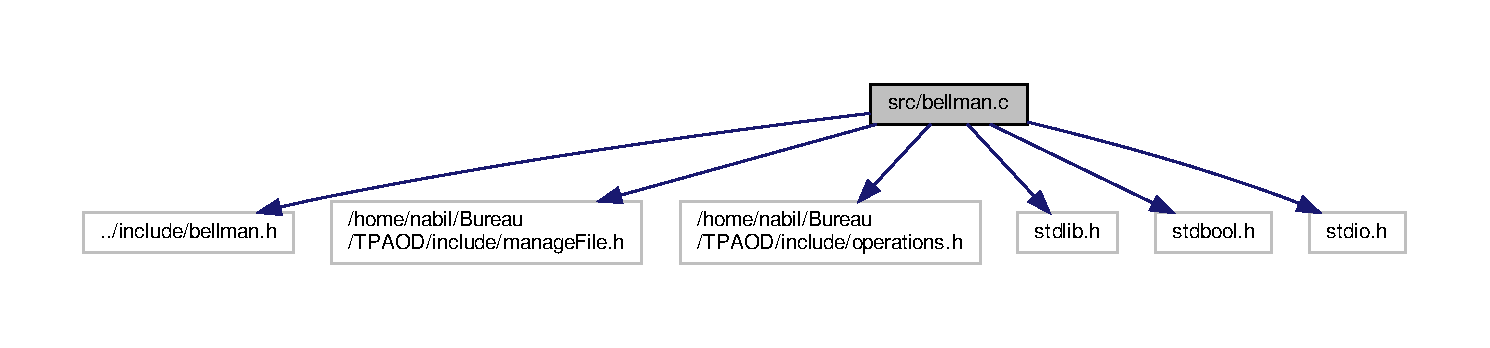
\includegraphics[width=350pt]{bellman_8c__incl}
\end{center}
\end{figure}
\subsection*{Functions}
\begin{DoxyCompactItemize}
\item 
int $\ast$$\ast$ \hyperlink{bellman_8c_ad90a646ea8e0c6b3896c902b909b237f}{initialiser} (int depi, int depj, int n, int m, char $\ast$$\ast$source, char $\ast$$\ast$target, int $\ast$lA, int $\ast$lB)
\begin{DoxyCompactList}\small\item\em la fonction crée une matrice des coûts Selon la modélisation récursive par équations de Bellman \end{DoxyCompactList}\end{DoxyCompactItemize}


\subsection{Detailed Description}
la création de la matrice des coûts 



\subsection{Function Documentation}
\mbox{\Hypertarget{bellman_8c_ad90a646ea8e0c6b3896c902b909b237f}\label{bellman_8c_ad90a646ea8e0c6b3896c902b909b237f}} 
\index{bellman.\+c@{bellman.\+c}!initialiser@{initialiser}}
\index{initialiser@{initialiser}!bellman.\+c@{bellman.\+c}}
\subsubsection{\texorpdfstring{initialiser()}{initialiser()}}
{\footnotesize\ttfamily int $\ast$$\ast$ initialiser (\begin{DoxyParamCaption}\item[{int}]{depi,  }\item[{int}]{depj,  }\item[{int}]{n,  }\item[{int}]{m,  }\item[{char $\ast$$\ast$}]{source,  }\item[{char $\ast$$\ast$}]{target,  }\item[{int $\ast$}]{lA,  }\item[{int $\ast$}]{lB }\end{DoxyParamCaption})}



la fonction crée une matrice des coûts Selon la modélisation récursive par équations de Bellman 


\begin{DoxyParams}{Parameters}
{\em depi} & c\textquotesingle{}est le départ de ligne liée au fichier f1 \\
\hline
{\em depi} & c\textquotesingle{}est le départ de ligne liée au fichier f2 \\
\hline
{\em n} & c\textquotesingle{}est la fin de ligne liée au fichier f1 \\
\hline
{\em m} & c\textquotesingle{}est la fin de ligne liée au fichier f2 \\
\hline
{\em source} & pointeur sur les lignes du fichier f1 \\
\hline
{\em target} & pointeur sur les lignes du fichier f2 \\
\hline
{\em lA} & tableau contenant les tailles du fichier f1 \\
\hline
{\em l\+B2} & tableau contenant les tailles du fichier f2 \\
\hline
\end{DoxyParams}

\hypertarget{computePatchOpt_8c}{}\section{src/compute\+Patch\+Opt.c File Reference}
\label{computePatchOpt_8c}\index{src/compute\+Patch\+Opt.\+c@{src/compute\+Patch\+Opt.\+c}}


le fichier main qui crée le patch  


{\ttfamily \#include \char`\"{}../include/compute\+Patch\+Opt.\+h\char`\"{}}\newline
Include dependency graph for compute\+Patch\+Opt.\+c\+:\nopagebreak
\begin{figure}[H]
\begin{center}
\leavevmode
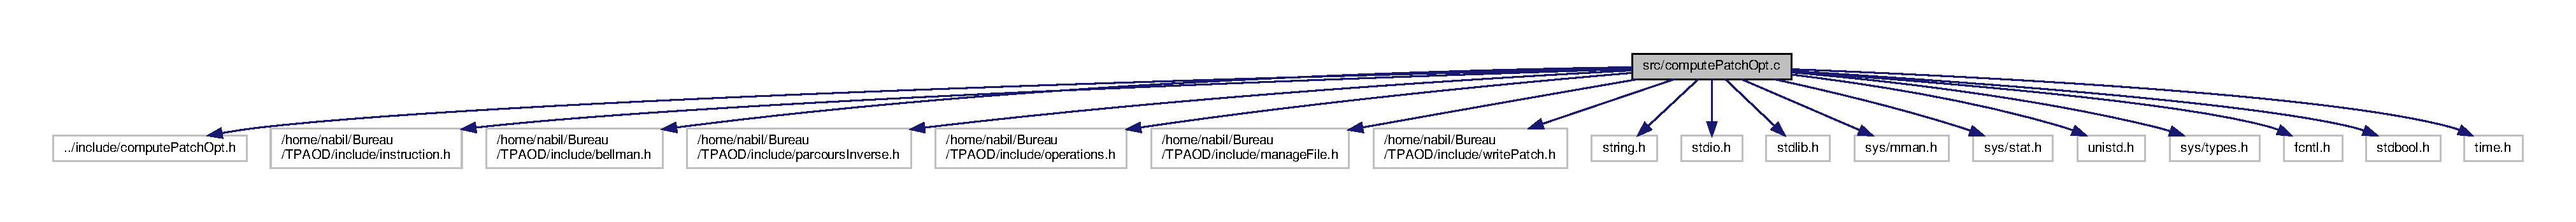
\includegraphics[width=350pt]{computePatchOpt_8c__incl}
\end{center}
\end{figure}
\subsection*{Functions}
\begin{DoxyCompactItemize}
\item 
\mbox{\Hypertarget{computePatchOpt_8c_a3c04138a5bfe5d72780bb7e82a18e627}\label{computePatchOpt_8c_a3c04138a5bfe5d72780bb7e82a18e627}} 
int {\bfseries main} (int argc, char $\ast$$\ast$argv)
\end{DoxyCompactItemize}


\subsection{Detailed Description}
le fichier main qui crée le patch 

\begin{DoxyAuthor}{Author}
\{B\+E\+N\+S\+R\+H\+I\+ER Nabil , Y\+A\+G\+O\+U\+TI Redouane\} 
\end{DoxyAuthor}
\begin{DoxyDate}{Date}
07/11/2019 
\end{DoxyDate}
\begin{DoxyVersion}{Version}
4.\+0 
\end{DoxyVersion}

\hypertarget{instruction_8c}{}\section{src/instruction.c File Reference}
\label{instruction_8c}\index{src/instruction.\+c@{src/instruction.\+c}}


le fichier contenant la structure sur laquelle on sauvegarde une instruction  


{\ttfamily \#include \char`\"{}../include/instruction.\+h\char`\"{}}\newline
{\ttfamily \#include $<$stdlib.\+h$>$}\newline
{\ttfamily \#include $<$stdio.\+h$>$}\newline
Include dependency graph for instruction.\+c\+:\nopagebreak
\begin{figure}[H]
\begin{center}
\leavevmode
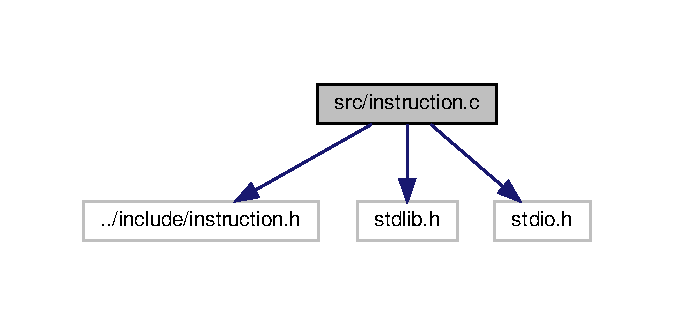
\includegraphics[width=324pt]{instruction_8c__incl}
\end{center}
\end{figure}
\subsection*{Functions}
\begin{DoxyCompactItemize}
\item 
struct instruction $\ast$ \hyperlink{instruction_8c_a86bf15e3b1449808698794dd91ead880}{get\+Head} (int seuil, int lignes, int colonnes, struct instruction $\ast$end, char $\ast$$\ast$source, char $\ast$$\ast$target, int $\ast$tab1, int $\ast$tab2)
\begin{DoxyCompactList}\small\item\em la fonction renvoie un pointeur vers l\textquotesingle{}instruction finale pour la ligne (0,0) \end{DoxyCompactList}\item 
\mbox{\Hypertarget{instruction_8c_a6c7c8ecbfe275db893726942290b4092}\label{instruction_8c_a6c7c8ecbfe275db893726942290b4092}} 
void {\bfseries remplir} (struct instruction $\ast$current, struct instruction $\ast$next, int i, int j)
\item 
void \hyperlink{instruction_8c_adfa5a4bf8e6e014cc0d1412009960d71}{free\+\_\+instructions} (struct instruction $\ast$current)
\begin{DoxyCompactList}\small\item\em libere la liste chainée des instructions. \end{DoxyCompactList}\end{DoxyCompactItemize}


\subsection{Detailed Description}
le fichier contenant la structure sur laquelle on sauvegarde une instruction 



\subsection{Function Documentation}
\mbox{\Hypertarget{instruction_8c_adfa5a4bf8e6e014cc0d1412009960d71}\label{instruction_8c_adfa5a4bf8e6e014cc0d1412009960d71}} 
\index{instruction.\+c@{instruction.\+c}!free\+\_\+instructions@{free\+\_\+instructions}}
\index{free\+\_\+instructions@{free\+\_\+instructions}!instruction.\+c@{instruction.\+c}}
\subsubsection{\texorpdfstring{free\+\_\+instructions()}{free\_instructions()}}
{\footnotesize\ttfamily void free\+\_\+instructions (\begin{DoxyParamCaption}\item[{struct instruction $\ast$}]{current }\end{DoxyParamCaption})}



libere la liste chainée des instructions. 


\begin{DoxyParams}{Parameters}
{\em $\ast$current} & l\textquotesingle{}instruction courante \\
\hline
\end{DoxyParams}
\mbox{\Hypertarget{instruction_8c_a86bf15e3b1449808698794dd91ead880}\label{instruction_8c_a86bf15e3b1449808698794dd91ead880}} 
\index{instruction.\+c@{instruction.\+c}!get\+Head@{get\+Head}}
\index{get\+Head@{get\+Head}!instruction.\+c@{instruction.\+c}}
\subsubsection{\texorpdfstring{get\+Head()}{getHead()}}
{\footnotesize\ttfamily struct instruction $\ast$ get\+Head (\begin{DoxyParamCaption}\item[{int}]{seuil,  }\item[{int}]{lignes,  }\item[{int}]{colonnes,  }\item[{struct instruction $\ast$}]{end,  }\item[{char $\ast$$\ast$}]{source,  }\item[{char $\ast$$\ast$}]{target,  }\item[{int $\ast$}]{tab1,  }\item[{int $\ast$}]{tab2 }\end{DoxyParamCaption})}



la fonction renvoie un pointeur vers l\textquotesingle{}instruction finale pour la ligne (0,0) 


\begin{DoxyParams}{Parameters}
{\em seuil} & la taille de ligne et colonne que la mémoire peut supporter \\
\hline
{\em lignes} & nombre de lignes du fichier f1 \\
\hline
{\em colonnes} & nombre de lignes du fichier f2 \\
\hline
{\em $\ast$end} & un pointeur vers une instruction \\
\hline
{\em sources} & pointeur sur les lignes du fichier f1 \\
\hline
{\em target} & pointeur sur les lignes du fichier f2 \\
\hline
{\em tab1} & tableau contenant les tailles du fichier f1 \\
\hline
{\em tab2} & tableau contenant les tailles du fichier f2 \\
\hline
\end{DoxyParams}

\hypertarget{manageFile_8c}{}\section{src/manage\+File.c File Reference}
\label{manageFile_8c}\index{src/manage\+File.\+c@{src/manage\+File.\+c}}


les outils nécessaires pour calculer le coût  


{\ttfamily \#include \char`\"{}../include/manage\+File.\+h\char`\"{}}\newline
{\ttfamily \#include \char`\"{}../include/operations.\+h\char`\"{}}\newline
{\ttfamily \#include $<$stdlib.\+h$>$}\newline
{\ttfamily \#include $<$string.\+h$>$}\newline
Include dependency graph for manage\+File.\+c\+:\nopagebreak
\begin{figure}[H]
\begin{center}
\leavevmode
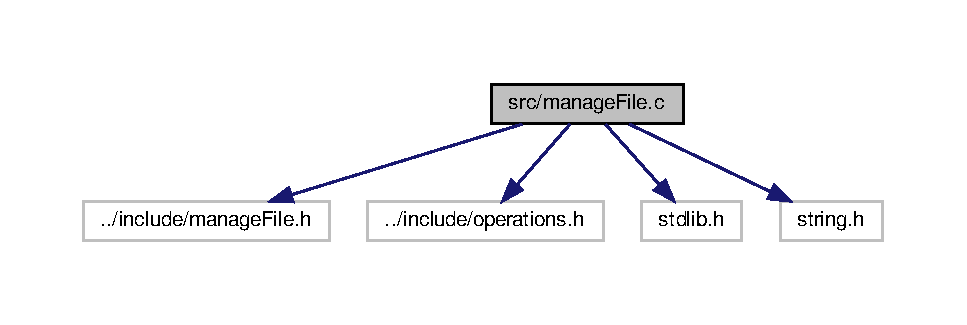
\includegraphics[width=350pt]{manageFile_8c__incl}
\end{center}
\end{figure}
\subsection*{Functions}
\begin{DoxyCompactItemize}
\item 
\mbox{\Hypertarget{manageFile_8c_aba9d72cb03b8fb4592eaef9165110bf9}\label{manageFile_8c_aba9d72cb03b8fb4592eaef9165110bf9}} 
int \hyperlink{manageFile_8c_aba9d72cb03b8fb4592eaef9165110bf9}{nb\+Line} (char $\ast$file, int size)
\begin{DoxyCompactList}\small\item\em renvoie le nombre de ligne dans un fichier. \end{DoxyCompactList}\item 
\mbox{\Hypertarget{manageFile_8c_af98375ccfdbc1f5472fc0180bc5bf18d}\label{manageFile_8c_af98375ccfdbc1f5472fc0180bc5bf18d}} 
int \hyperlink{manageFile_8c_af98375ccfdbc1f5472fc0180bc5bf18d}{cout} (int i, int j, char $\ast$$\ast$source, char $\ast$$\ast$target, int $\ast$tab1, int $\ast$tab2)
\begin{DoxyCompactList}\small\item\em calcul le coût (i,j) \end{DoxyCompactList}\item 
\mbox{\Hypertarget{manageFile_8c_ae94673caf99b110e72f8d8e0f8c8b6aa}\label{manageFile_8c_ae94673caf99b110e72f8d8e0f8c8b6aa}} 
int $\ast$ \hyperlink{manageFile_8c_ae94673caf99b110e72f8d8e0f8c8b6aa}{longeur\+File} (char $\ast$file, int size, int line\+Nb)
\begin{DoxyCompactList}\small\item\em liste des tailles des lignes d\textquotesingle{}un fichier en paramètres \end{DoxyCompactList}\item 
\mbox{\Hypertarget{manageFile_8c_a66e4fc320366a3fd19fd6d3d5b962fac}\label{manageFile_8c_a66e4fc320366a3fd19fd6d3d5b962fac}} 
char $\ast$$\ast$ \hyperlink{manageFile_8c_a66e4fc320366a3fd19fd6d3d5b962fac}{pointeur\+Ligne} (char $\ast$file, int $\ast$tab, int len)
\begin{DoxyCompactList}\small\item\em liste des pointeurs sur chaque début de ligne \end{DoxyCompactList}\end{DoxyCompactItemize}


\subsection{Detailed Description}
les outils nécessaires pour calculer le coût 


\hypertarget{operations_8c}{}\section{src/operations.c File Reference}
\label{operations_8c}\index{src/operations.\+c@{src/operations.\+c}}


les opérations nécessaires pour faire le calcul  


{\ttfamily \#include \char`\"{}../include/operations.\+h\char`\"{}}\newline
{\ttfamily \#include $<$stdlib.\+h$>$}\newline
Include dependency graph for operations.\+c\+:\nopagebreak
\begin{figure}[H]
\begin{center}
\leavevmode
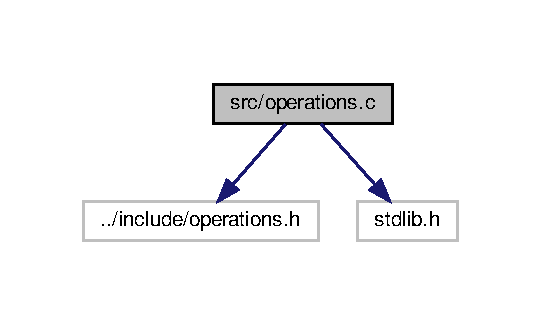
\includegraphics[width=260pt]{operations_8c__incl}
\end{center}
\end{figure}
\subsection*{Functions}
\begin{DoxyCompactItemize}
\item 
\mbox{\Hypertarget{operations_8c_a836f3054199c73ee9fa1873153aace86}\label{operations_8c_a836f3054199c73ee9fa1873153aace86}} 
int \hyperlink{operations_8c_a836f3054199c73ee9fa1873153aace86}{index\+Min} (int $\ast$tab, int tab\+Size)
\begin{DoxyCompactList}\small\item\em renvoie l\textquotesingle{}indice du minimum \end{DoxyCompactList}\item 
\mbox{\Hypertarget{operations_8c_a273c89211eebcaf824d2649fc93548a2}\label{operations_8c_a273c89211eebcaf824d2649fc93548a2}} 
int \hyperlink{operations_8c_a273c89211eebcaf824d2649fc93548a2}{min} (int i, int j, int k)
\begin{DoxyCompactList}\small\item\em renvoie le minimum \end{DoxyCompactList}\item 
\mbox{\Hypertarget{operations_8c_a7aaf2c5d74d44df845fa1236badf4dfa}\label{operations_8c_a7aaf2c5d74d44df845fa1236badf4dfa}} 
int \hyperlink{operations_8c_a7aaf2c5d74d44df845fa1236badf4dfa}{max} (int i, int j)
\begin{DoxyCompactList}\small\item\em renvoie le maximum \end{DoxyCompactList}\end{DoxyCompactItemize}


\subsection{Detailed Description}
les opérations nécessaires pour faire le calcul 


\hypertarget{parcoursInverse_8c}{}\section{src/parcours\+Inverse.c File Reference}
\label{parcoursInverse_8c}\index{src/parcours\+Inverse.\+c@{src/parcours\+Inverse.\+c}}


Création d\textquotesingle{}une liste chainée des instructions du patch.  


{\ttfamily \#include \char`\"{}../include/parcours\+Inverse.\+h\char`\"{}}\newline
{\ttfamily \#include $<$stdbool.\+h$>$}\newline
{\ttfamily \#include $<$stdlib.\+h$>$}\newline
{\ttfamily \#include $<$stdio.\+h$>$}\newline
Include dependency graph for parcours\+Inverse.\+c\+:\nopagebreak
\begin{figure}[H]
\begin{center}
\leavevmode
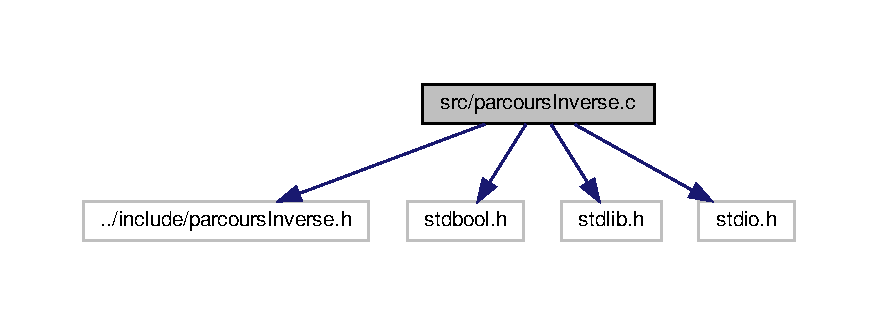
\includegraphics[width=350pt]{parcoursInverse_8c__incl}
\end{center}
\end{figure}
\subsection*{Functions}
\begin{DoxyCompactItemize}
\item 
struct instruction $\ast$ \hyperlink{parcoursInverse_8c_a0a8ded8f236c70a62ebf1f0932d2d264}{court\+Chemin} (int depi, int depj, struct instruction $\ast$end, int n, int m, int $\ast$$\ast$matrix, char $\ast$$\ast$pA, char $\ast$$\ast$pB, int $\ast$lA, int $\ast$lB)
\begin{DoxyCompactList}\small\item\em la fonction crée une liste chainée des instructions à faire à travers la matrice des coûts passée en paramètre \end{DoxyCompactList}\end{DoxyCompactItemize}


\subsection{Detailed Description}
Création d\textquotesingle{}une liste chainée des instructions du patch. 



\subsection{Function Documentation}
\mbox{\Hypertarget{parcoursInverse_8c_a0a8ded8f236c70a62ebf1f0932d2d264}\label{parcoursInverse_8c_a0a8ded8f236c70a62ebf1f0932d2d264}} 
\index{parcours\+Inverse.\+c@{parcours\+Inverse.\+c}!court\+Chemin@{court\+Chemin}}
\index{court\+Chemin@{court\+Chemin}!parcours\+Inverse.\+c@{parcours\+Inverse.\+c}}
\subsubsection{\texorpdfstring{court\+Chemin()}{courtChemin()}}
{\footnotesize\ttfamily struct instruction $\ast$ court\+Chemin (\begin{DoxyParamCaption}\item[{int}]{depi,  }\item[{int}]{depj,  }\item[{struct instruction $\ast$}]{end,  }\item[{int}]{n,  }\item[{int}]{m,  }\item[{int $\ast$$\ast$}]{matrix,  }\item[{char $\ast$$\ast$}]{pA,  }\item[{char $\ast$$\ast$}]{pB,  }\item[{int $\ast$}]{lA,  }\item[{int $\ast$}]{lB }\end{DoxyParamCaption})}



la fonction crée une liste chainée des instructions à faire à travers la matrice des coûts passée en paramètre 


\begin{DoxyParams}{Parameters}
{\em depi} & c\textquotesingle{}est le départ de ligne liée au fichier f1 \\
\hline
{\em depi} & c\textquotesingle{}est le départ de ligne liée au fichier f2 \\
\hline
{\em end} & c\textquotesingle{}est l\textquotesingle{}insruction donnée de la derniere opération du cour chemin \\
\hline
{\em n} & c\textquotesingle{}est la fin de ligne liée au fichier f1 \\
\hline
{\em m} & c\textquotesingle{}est la fin de ligne liée au fichier f2 \\
\hline
{\em pA} & pointeur sur les lignes du fichier f1 \\
\hline
{\em pB} & pointeur sur les lignes du fichier f2 \\
\hline
{\em lA} & tableau contenant les tailles du fichier f1 \\
\hline
{\em l\+B2} & tableau contenant les tailles du fichier f2 \\
\hline
\end{DoxyParams}
si on finit les éléments du fichier target on détruit le reste du fichier source

par contre si on finit les éléments du fichier source on ajoute le reste du fichier target

par contre si on finit les éléments du fichier source on ajoute le reste du fichier target
\hypertarget{writePatch_8c}{}\section{src/write\+Patch.c File Reference}
\label{writePatch_8c}\index{src/write\+Patch.\+c@{src/write\+Patch.\+c}}


le fichier prend les arguments nécessaires pour écrire le patch  


{\ttfamily \#include \char`\"{}../include/write\+Patch.\+h\char`\"{}}\newline
{\ttfamily \#include $<$stdlib.\+h$>$}\newline
Include dependency graph for write\+Patch.\+c\+:\nopagebreak
\begin{figure}[H]
\begin{center}
\leavevmode
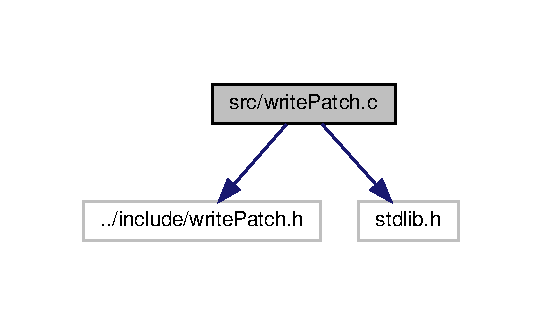
\includegraphics[width=260pt]{writePatch_8c__incl}
\end{center}
\end{figure}
\subsection*{Functions}
\begin{DoxyCompactItemize}
\item 
\mbox{\Hypertarget{writePatch_8c_a136f3354672680ef82cbe8419df0863f}\label{writePatch_8c_a136f3354672680ef82cbe8419df0863f}} 
void {\bfseries print\+\_\+string} (F\+I\+LE $\ast$file, char $\ast$s, int len)
\item 
void \hyperlink{writePatch_8c_ae4d0ae4520c23390909bd39be686d751}{write\+\_\+patch} (F\+I\+LE $\ast$file, struct instruction $\ast$instruction, int $\ast$tab1, int $\ast$tab2)
\begin{DoxyCompactList}\small\item\em la fonction écrire l\textquotesingle{}instruction donnée en parametre \end{DoxyCompactList}\end{DoxyCompactItemize}


\subsection{Detailed Description}
le fichier prend les arguments nécessaires pour écrire le patch 



\subsection{Function Documentation}
\mbox{\Hypertarget{writePatch_8c_ae4d0ae4520c23390909bd39be686d751}\label{writePatch_8c_ae4d0ae4520c23390909bd39be686d751}} 
\index{write\+Patch.\+c@{write\+Patch.\+c}!write\+\_\+patch@{write\+\_\+patch}}
\index{write\+\_\+patch@{write\+\_\+patch}!write\+Patch.\+c@{write\+Patch.\+c}}
\subsubsection{\texorpdfstring{write\+\_\+patch()}{write\_patch()}}
{\footnotesize\ttfamily void write\+\_\+patch (\begin{DoxyParamCaption}\item[{F\+I\+LE $\ast$}]{file,  }\item[{struct instruction $\ast$}]{instruction,  }\item[{int $\ast$}]{tab1,  }\item[{int $\ast$}]{tab2 }\end{DoxyParamCaption})}



la fonction écrire l\textquotesingle{}instruction donnée en parametre 


\begin{DoxyParams}{Parameters}
{\em file} & le fichier surlequelle on écrit \\
\hline
{\em instruction} & c\textquotesingle{}est l\textquotesingle{}insruction donnée \\
\hline
{\em tab1} & tableau contenant les tailles du fichier f1 \\
\hline
{\em tab2} & tableau contenant les tailles du fichier f2 \\
\hline
\end{DoxyParams}

%--- End generated contents ---

% Index
\backmatter
\newpage
\phantomsection
\clearemptydoublepage
\addcontentsline{toc}{chapter}{Index}
\printindex

\end{document}
